\chapter{Preliminary Work}

\matteo{I'm pretty sure you can merge this stuff in the previous chapter; move sanitizers up and move info on each fuzzing framework with its respective section}

\section{Understanding OSS-Fuzz projects}
To be accepted by OSS-Fuzz, the developers create a "pull request" to the OSS-Fuzz repository, but only projects that are relevant and/or critical to the global IT infrastructure with a significant user base will be integrated.
\newline \newline
To check if your project is eligible for OSS-Fuzz, Google provides a mathematical formula to calculate the "Open-Source Project Criticality Score" \cite{score} in a range between 0 \textit{(least critical)} and 1 \textit{(most critical)}, which is the following:
\ \\
\begin{equation}
    CriticalityScore = \frac{1}{\sum \alpha_i}\  \sum_i \alpha_i \ \frac{\log(1+S_i)}{\log(1+\max(S_i,T_i))}
\end{equation}
\ \\
The parameters evaluated are the followings:
\begin{itemize}
    \item \textbf{created-since} ($\alpha_i = 1$, $T_i = 120$): months since the project was created
    \item \textbf{updated-since} ($\alpha_i = -1$, $T_i = 120$): months since the project was last updated
    \item \textbf{contributor-count} ($\alpha_i = 2$, $T_i = 5000$): count of commits made by distinct contributors
    \item \textbf{org-count} ($\alpha_i = 1$, $T_i = 10$): count of distinct organizations contributing to the project
    \item \textbf{commit-frequency} ($\alpha_i = 1$, $T_i = 1000$): average number of commits per week in the last year
    \item \textbf{recent-releases-count} ($\alpha_i = 0.5$, $T_i = 26$): number of releases in the last year
    \item \textbf{closed-issues-count} ($\alpha_i = 0.5$, $T_i = 5000$): number of issues closed in the last 90 days
    \item \textbf{updated-issues-count} ($\alpha_i = 0.5$, $T_i = 5000$): number of issues updated in the last 90 days
    \item \textbf{comment-frequency} ($\alpha_i = 1$, $T_i = 15$): average number of comments per issue in the last 90 days
    \item \textbf{dependents-count} ($\alpha_i = 2$, $T_i = 500000$): number of project mentions in the commit messages
\end{itemize}
\ \\
Only projects scoring a value $\geq 0.7$ may be eligible to be integrated in the OSS-Fuzz campaign.

\newpage
The main file structure of an OSS-Fuzz project is composed by 3 files.
\newline \newline
The \textit{project.yaml} configuration file stores project metadata needed by OSS-Fuzz to correctly provide its services, including:
\begin{itemize}
    \item \textbf{homepage:} url to the project's homepage
    \item \textbf{language:} programming language used to write the project (C, C++, Go, Rust, Python, JVM languages, Swift)
    \item \textbf{primary\_contacts:} list of email addresses that will be automatically CCed on crash reports and fuzzer statistics
    \item \textbf{main\_repo:} path to the source code repository hosting the project
    \item \textbf{vendor\_ccs:} \textit{optional}, list of vendors' email addresses that want access to the bug reports
    \item \textbf{sanitizers:} \textit{optional}, list of sanitizers that are available on the project (address, undefined, memory), if not specified "address" and "undefined" will be used
    \item \textbf{architectures:} \textit{optional}, list of architectures that can build the project (supported only x86\_64 and i386)
    \item \textbf{fuzzing\_engines:} \textit{optional}, list of fuzzing engines available (libfuzzer, afl, honggfuzz and centipede), if not specified "libfuzzer" will be used
    \item \textbf{help\_url:} \textit{optional}, used on reports to provide a custom guide related to bug reproduction steps
    \item \textbf{builds\_per\_day:} \textit{optional}, number of times a project should be built per day, OSS-Fuzz allows up to 4 builds per day and builds once per day by default
    \item \textbf{file\_github\_issue:} \textit{optional}, mirrors OSS-Fuzz bug reports on the project's GitHub repository via "Issues"
\end{itemize}
\ \\
The \textit{Dockerfile} defines a container with all the dependencies and resources needed to build the project and prepare the testing environment.
\newline
To avoid having developers create and maintain their own customized Docker containers and create an homogeneous and standard environment, OSS-Fuzz provides several "base images" for each supported language, built on top of Ubuntu 20.04 and with the appropriate compilers and toolchains already installed.
\newline
After pulling the most appropriate base image, there are usually several "apt-get" and "git clone" commands related to downloading and installing all the required packages and dependencies needed to correctly build the project.
\newline
Finally, the build script and any other fuzzer files are pulled from the project's repository.
\newline \newline
The \textit{build.sh:} script, executed inside the Docker container, performs all the operations necessary to build the project and the fuzzing targets that will be tested.
\newline
In general, the script should build the project and the fuzz targets using the correct compiler and appropriate compiler flags.
\newline
To provide a more flexible and accessible build system, the Docker image provides several environment variables regarding directory locations, compilers and compiling flags, allowing developers to easily re-target scripts with little effort.




\newpage
\section{Understanding FuzzBench benchmarks}
Explain what is a project in FuzzBench...
\newline \newline
Explain the structure of a project and its files...
\newline \newline
Explain the commands from the "gsutil" suite...




\newpage
\section{Sanitizers} \label{sanitizers}
A \textit{code sanitizer} is a tool used to detect bugs in a program during both compilation and runtime, and this is done by "instrumenting" the code.
\newline
The act of "instrumentation" refers to modifying either the source code or binary code that is being compiled to add some additional functionalities and references that can be used by other tools to perform code analysis, logging or profiling.
\newline
It's important to notice that this process is not only severely limited by the single execution flow analyzed, but also introduces a non-trivial overhead both in terms of increased execution time and memory usage, which may cause problems when it comes to managing computing resources.
\newline \newline
Although code sanitizers should be a standard practice in the development cycle of a program, unfortunately this is not the case as introducing these tools not only requires extensive tests to check for potential errors, but also because they do not always interact very well with shared libraries or other external dependencies.
\newline
It is also extremely important to mention that these bug detection tools are not meant to be linked against production executables, as their runtime was not developed with security-sensitive constraints and may compromise the security of the released product. \cite{asan_docs}\cite{msan_docs}\cite{ubsan_docs}
\newline \newline
In this thesis, we focused on using several sanitizers developed by Google \cite{san_repo} as part of its tools available to open-source developers to improve their programs and make them more secure, which proved to be particularly effective when combined with fuzzing due to its ability to trigger bugs.


\ \\
\subsection{ASan and LSan}
The \textit{Address Sanitizer} \cite{serebryany2012addresssanitizer} is a memory error detection tool for C/C++ that helps developers to find and fix any out-of-bounds accesses to heap, stack and global objects as well as use-after-free bugs, and its one of the most widely used and effective sanitizers.
\newline \newline
It works by using a shadow memory to map the memory regions allocated by the application and record whether each byte of such areas can be safely accessed by load/store operations. Each memory region is assigned a shadow counterpart, containing metadata about its size and the offset range that can be used to safely access it, while any attempt to read/write beyond such boundaries will trigger a sanitizer error, as shown by the figure below:
\newline
\begin{figure}[h]
\centering
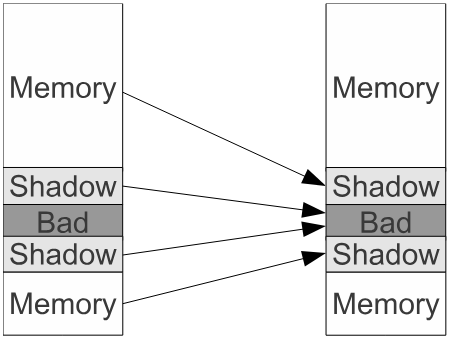
\includegraphics[scale=0.4]{foto/shadow_memory.png}
\caption{Memory mapping of ASan \cite{serebryany2012addresssanitizer}}
\label{fig:asan_shadow}
\end{figure}
\newline
Detection of out-of-bounds accesses to globals and stack objects is done in a similar way, which means by creating poisoned memory regions around such objects: \textit{global variables} are poisoned at compile-time and their addresses computed during the application startup, while \textit{stack objects} are poisoned and recorded at run-time.
\newline \newline
The management of the shadow memory is done by ASan run-time library, containing specialized implementation of the \verb|malloc| and \verb|free| functions, which allocate extra memory for shadow and poisoned memory zones as well as keeping a FIFO stack of allocated and freed memory regions to detect use-after-free, double-free and invalid-free bugs.
\newline \newline
Finally, ASan adds a slight overhead, increasing execution times by an average 170\% and memory usage by 3.4x.
\newline \newline \newline
Another component is the \textit{Leak Sanitizer} (or \textit{LSan}), a memory leak detector enabled by default in ASan that returns which portions of the program are leaking memory as well as the size leaked, thanks to comprehensive and exhaustive stack traces. Although this tool may seem very helpful, it usually generate huge logs especially when having complex programs that heavily rely on external libraries, which oftentimes do not perform clean releases of the objects used.


\ \\
\subsection{MSan}
The \textit{Memory Sanitizer} \cite{stepanov2015memorysanitizer} is a memory reads detector for C/C++ that helps developers to find and fix use-of-uninitialized-memory (UUM) bugs.
The C and C++ languages usually create uninitialized stack and heap objects (unless \verb|calloc| is invoked), and discovering these bugs can be quite tricky as they do not necessarily occur in every execution and could be triggered by any operation performed by the program.
\newline \newline
It works by using a shadow memory to map each bit of application memory and encode its state (0 initialized, 1 otherwise): all newly allocated memory is poisoned, i.e. the corresponding shadow memory is initialized to \verb|0xFF|, and "shadow propagation" operations are performed to safely copy an uninitialized variable between memory regions as well as simple logic and arithmetic operations without occurring in errors.
\newline
Performing a load operation from uninitialized memory returns an \textit{undefined value}, and operations like conditional branch, syscall and pointer dereference are most likely to trigger UUM bugs.
\newline
\begin{figure}[h]
\centering
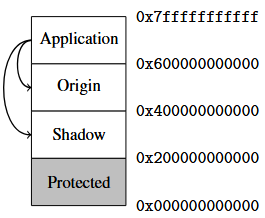
\includegraphics[scale=0.63]{foto/shadow_memory_2.png}
\caption{Memory mapping of MSan \cite{stepanov2015memorysanitizer}}
\label{fig:msan_shadow}
\end{figure}
\newline
Given that UUM bugs are notoriously hard to reproduce and debug, the "origin-tracking-mode" can be used to obtain more comprehensive stack-traces and helping the developer to understand where it should have happened, although it relies on the program's symbols to provide meaningful information.
\newline
If necessary, there is also an "advanced-origin-tracking-mode", printing the stack traces of all operations from the allocation of the uninitialized variable up to its load, but its usability is still discussed due to the huge amount of memory it requires.
\newline \newline
The management of the shadow memory is done by MSan run-time library, that maps the "shadow" and (optional) "origin" areas and marks as uninitialized any new allocated regions as well as the deallocated ones. To update the shadow region, a large subset of the standard \verb|libc| functions are intercepted.
\newline \newline
Fixing UUM bugs is generally a quick task, like initializing the memory region using appropriate functions or simply setting all bytes to 0, but many developers avoid this sanitizer due to the huge slowdown that it introduces.
\newline
In fact MSan adds a modest overhead, increasing execution times by an average 300\% and memory usage by 2x on short programs, values that rapidly worsen with complex programs and when "origin-tracking-mode" is enabled.


\ \\
\subsection{UBSan}
The \textit{Undefined Behavior Sanitizer} \cite{ubsan_docs} is a fast undefined-behavior detector for C/C++, that helps developers to find and fix undefined-behavior (UB) bugs.
\newline
Common operations that may lead to undefined behaviors are: array subscription out of bounds, overflows/underflows originating from mathematical or logical operations, dereferenced, misagnlied or null pointers and conversion between data types.
\newline \newline
By default, due to its simplistic nature, the tool does not print stack-traces and uses a minimal run-time library. If needed, "print-stacktrace-mode" can be enabled to obtain more comprehensive results, although it relies on the program’s symbols to provide meaningful information.
\newline \newline
Finally, UBSan adds a trivial overhead, increasing execution times by an average 120\% and memory usage by 2x.






\newpage
\section{Setting up the environment}

\matteo{Nice, we need this info. Maybe we should shift it at the end of "methodology", or at the start of "results", see which seems better}
All tests were performed on two separate machines, both equipped with personal installations of Ubuntu 22.04 LTS, already run-in and used.
\newline \newline \newline
Regarding tools for general purpose, I used Docker, Valgrind, Python 3, gsutil and Google Chrome.
\newline \newline
The \textit{Docker} application was needed to run the different containers needed by OSS-Fuzz to build the projects and run the tests.
\newline \newline
\textit{Valgrind} \cite{valgrind} is an instrumentation framework to perform memory analysis, profiling and management during the execution of a program.
More specifically, it was used to perform memory analysis in projects built without sanitizers.
\newline \newline
The \textit{Python 3} language was used to create several scripts that I used to perform information scraping, reports analysis and bug deduplication.
It is also used by OSS-Fuzz to provide some functionalities, and this will be discussed later. 
\newline \newline
The \textit{gsutil} suite is a command-line tool provided by Google to access resources stored on Google Cloud Service from your local machine, and it was used to analyze the FuzzBench benchmarks and download other resources.
\newline \newline
Finally, \textit{Google Chrome} and its "development driver" were needed during the information scraping phase of this work, discussed in section \ref{selection}.
\newline \newline \newline
Regarding \textit{OSS-Fuzz}, most of the work was done on its GitHub repository, which I cloned locally on both machines.
\newline
To provide its services, OSS-Fuzz uses several python scripts that can be invoked via command-line using appropriate arguments. These commands can be used to update the projects' files and projects' images, build the project's image and its fuzzers but also download resources like corpora. 
\newline \newline \newline
Regarding \textit{FuzzBench} [...]

